\section{An LQG / Riccati alternative we examined and discarded}\label{app:lqg}

The body of these notes is built around the SMC${}^2$ filter and
controller of Sections~\ref{sec:pf}--\ref{sec:mpc}: a non-linear,
sample-based machinery aimed at the cubic Stuart--Landau dynamics of
FSA-v2. For completeness we also examined the natural linear
alternative -- a linear--quadratic--Gaussian controller solved by a
backward differential Riccati equation -- and benchmarked it against
the SMC${}^2$ MPC. This appendix records what that alternative looks
like, what it requires, and why it does not match the
non-linear machinery on this plant. The headline finding is that the
cubic Stuart--Landau term sits at the heart of FSA-v2's control
behaviour; any controller derived from a first-order linearisation
necessarily discards exactly the structure the project is designed
to exploit.

This appendix is included for the reader who wants the details. The
main text (Sections~\ref{sec:mpc-lqg-pointer},
\ref{sec:results-stage-i}, \ref{sec:discussion-lqg-pointer}) makes only
the brief reference required to honour the comparison.

\subsection{Three assumptions and the linearised problem}\label{app:lqg-A1A3}

Three assumptions reduce the FSA-v2 control problem to one with a
closed-form optimal feedback law.

\begin{assumption}\label{ass:lqg-A1}
There is a nominal trajectory $(x^*(t),\Phi^*(t))$ on $[0,T]$, taken in
the simplest case to be the deterministic-skeleton equilibrium
$(B^*,F^*,A^*)(\Phi_{\mathrm{const}})$ under a constant control. With
$\tilde x = x - x^*$ and $\tilde \Phi = \Phi - \Phi^*$, define the
linearised drift coefficients
\begin{equation}
  A_{\mathrm{lin}}(t) = \frac{\partial f}{\partial x}\bigg|_{*},
  \qquad B_{\mathrm{lin}}(t) = \frac{\partial f}{\partial \Phi}\bigg|_{*},
  \label{eq:lqg-AB}
\end{equation}
where $f$ is the drift of \eqref{eq:fsa-B}--\eqref{eq:fsa-A}.
\end{assumption}

The cubic Stuart--Landau term $-\eta A^3$ is linearised away under
Assumption~\ref{ass:lqg-A1}, so the bistable / limit-cycle behaviour
of the autonomic amplitude is lost. The linearisation is valid only
in a neighbourhood of the operating point.

\begin{assumption}\label{ass:lqg-A2}
The state-dependent Jacobi and CIR diffusions in
\eqref{eq:fsa-B}--\eqref{eq:fsa-A} are replaced by constant-coefficient
Gaussian noise $\bar\sigma\,\dd W$ evaluated at the operating point.
\end{assumption}

The $[0,1]$ and $[0,\infty)$ state constraints are no longer enforced
implicitly by the noise vanishing at the boundary, so trajectories may
leave the physiological domain. Acceptable when fluctuations around
the operating point are small relative to the boundary distances.

\begin{assumption}\label{ass:lqg-A3}
The cost \eqref{eq:cost} is replaced by the quadratic surrogate
\begin{equation}
  J_{\mathrm{LQ}}(\tilde \Phi)
    \;=\; \E\!\left[\,\int_0^T \bigl(\tilde x^{\!\top} Q \tilde x
                       + \tilde \Phi^{\!\top} R \tilde \Phi\bigr)\,\dd t
                       + \tilde x(T)^{\!\top} Q_T \tilde x(T)\,\right],
  \label{eq:lqg-cost}
\end{equation}
with $Q \succeq 0$, $R \succ 0$, $Q_T \succeq 0$.
\end{assumption}

To approximate the $-\!\int A\,\dd t$ reward, one chooses
$x_{\mathrm{ref}} \neq x^*$ shifted toward higher $A$ and penalises
$\tilde x = x - x_{\mathrm{ref}}$ with $Q$ giving most weight to the
$A$ component; this preserves $Q \succeq 0$. The soft fatigue barrier
$\lambda_F \cdot \max(F-\Fmax,0)^2$ is replaced by a quadratic in
$F-F^*$, which penalises both directions symmetrically -- too
restrictive on the rest side and too lax on the over-fatigue side
near the barrier.

\subsection{The differential Riccati equation}\label{app:lqg-riccati}

Under Assumptions~\ref{ass:lqg-A1}--\ref{ass:lqg-A3}, the optimal
feedback law for the linearised system is the time-varying linear
policy
\begin{equation}
  \tilde \Phi^*(t) \;=\; -K(t)\,\tilde x(t),
  \qquad K(t) \;=\; R^{-1}\,B_{\mathrm{lin}}(t)^{\!\top}\,P(t),
  \label{eq:lqg-feedback}
\end{equation}
where $P:[0,T] \to \R^{3\times 3}$, $P(t) \succeq 0$, solves the
\emph{differential Riccati equation}
\begin{equation}
  -\dot P(t) \;=\; A_{\mathrm{lin}}(t)^{\!\top} P(t)
                   + P(t)\,A_{\mathrm{lin}}(t)
                   - P(t)\,B_{\mathrm{lin}}(t)\,R^{-1}\,
                     B_{\mathrm{lin}}(t)^{\!\top} P(t)
                   + Q,
  \qquad P(T) = Q_T.
  \label{eq:riccati}
\end{equation}
Under
Assumptions~\ref{ass:lqg-A1}--\ref{ass:lqg-A2} the state-estimation
problem also linearises and is solved by the Kalman--Bucy filter; the
LQG controller is then the certainty-equivalent composition of
Kalman--Bucy filter and LQR feedback, and the (linear-Gaussian)
separation principle holds.

\paragraph{Implementation.}
Stage~H of the project provides this in
\texttt{smc2fc/control/lqg/}: \texttt{linearize.py} (JAX
\texttt{jacfwd} at the operating point), \texttt{riccati.py}
(fourth-order Runge--Kutta backward integrator on the project's outer
grid), and \texttt{controller.py} (\texttt{LQGController} emitting
both an open-loop schedule and a closed-loop feedback gain).
\texttt{version\_2/tools/bench\_lqg\_baseline\_fsa.py} mirrors the
SMC${}^2$ checkpoint schema for direct comparison.

\subsection{Three structural facts of the linearisation}\label{app:lqg-facts}

At the operating point $(B_{\mathrm{typ}},F_{\mathrm{typ}},A_{\mathrm{typ}},\Phi=1)$
the JAX-autodiff linearisation produces
\begin{equation}
  A_{\mathrm{lin}} =
  \begin{pmatrix}
   -0.024 & \phantom{-}0.000 & \phantom{-}0.005 \\
    0.000 & -0.157 & -0.029 \\
    0.030 & -0.026 & -0.007
  \end{pmatrix},
  \quad
  B_{\mathrm{lin}} =
  \begin{pmatrix} 0.0125 \\ 0.0300 \\ 0.0000 \end{pmatrix},
  \label{eq:lqg-numbers}
\end{equation}
with eigenvalues of $A_{\mathrm{lin}}$ approximately
$\{+0.003,\,-0.029,\,-0.162\}$. Three structural facts emerge.

\begin{enumerate}
  \item[(S1)] $B_{\mathrm{lin}}^{(A)} = 0$. The training stimulus
    $\Phi$ has \emph{no direct linear path} to the autonomic amplitude
    $A$. Linearised LQG can only steer $A$ via the slow detour
    $\Phi \to F \to A$.
  \item[(S2)] One eigenvalue of $A_{\mathrm{lin}}$ is positive
    ($+0.003$). At $A_{\mathrm{typ}} = 0.10$ the cubic damping
    $-\eta A^3$ contributes only
    $3\eta A_{\mathrm{typ}}^2 = 0.006$ to the $A$-direction rate, less
    than the destabilising contribution from the $\mu$-coupling. The
    linearisation is therefore \emph{unstable} in a slow $A$-direction;
    the cubic non-linearity that restores stability in the true model
    is not present in the linearised state space.
  \item[(S3)] $A_{\mathrm{lin}}^{(A,F)} = -0.026 < 0$. In the
    linearised state space, raising $F$ \emph{reduces} $A$, the
    \emph{opposite} of the true plant's coupling (raising $F$ raises
    $A$ via the slow build of $\mu$ before the quadratic suppression
    takes over). The first-order Taylor expansion at $A_{\mathrm{typ}}$
    inverts the sign of the physiologically relevant cross-coupling.
\end{enumerate}

No choice of $(Q,R,Q_T,x_{\mathrm{ref}})$ within the LQG family can
correct these structural facts -- they are what
Assumption~\ref{ass:lqg-A1} produces. Together they explain why the
LQG controller fails to match the SMC${}^2$ MPC: it is operating on a
state space whose connectivity, stability, and even sign of cross-coupling
have been replaced by their first-order Taylor surrogates at a point
where the true non-linearity dominates.

\subsection{Empirical comparison}\label{app:lqg-results}

The cost weights selected by a $T = 42$ d sweep are
$Q = \diag(0,100,100)$, $R = 1$, $Q_T = 0$,
$x_{\mathrm{ref}} = (B_0, 0.20, 0.30)^{\!\top}$,
$\Phi_{\mathrm{ref}} = 1$, clipped to $[0,3]$. The full Stage~H sweep
across horizons $T \in \{14,28,42,56,84\}$ days runs the LQG
schedule on the true non-linear FSA-v2 plant
(\texttt{StepwisePlant}); the resulting mean autonomic amplitude is
compared to the constant-$\Phi=1$ baseline on the same plant.

\begin{table}[h]
\centering
\small
\begin{tabular}{@{}rcrrrrr@{}}
\toprule
$T$ (d) & $h$ (min) & $\bar A_{\mathrm{LQG}}$ & $\bar A_{\mathrm{const}}$
   & ratio & F-viol & wall-clock \\
\midrule
$14$ & $15$ & $0.0830$ & $0.0824$ & $1.008$ & $0.00\%$ & $1.3$ s \\
$28$ & $15$ & $0.0944$ & $0.0943$ & $1.002$ & $0.00\%$ & $1.5$ s \\
$42$ & $15$ & $0.1450$ & $0.1396$ & $\mathbf{1.039}$ & $0.00\%$ & $1.6$ s \\
$56$ & $15$ & $0.2726$ & $0.2306$ & $\mathbf{1.182}$ & $0.00\%$ & $1.8$ s \\
$84$ & $15$ & $0.4258$ & $0.4442$ & $\mathbf{0.958}$ & $\mathbf{10.23\%}$ & $1.9$ s \\
\bottomrule
\end{tabular}
\caption{Tuned LQG performance against the constant-$\Phi=1$
baseline across horizons. The LQG schedule outperforms baseline by
$0$--$18\%$ with no fatigue-barrier violation up to $T = 56$ d; at
$T = 84$ d it underperforms baseline (ratio $0.96$) and produces
$10.23\%$ F-violation. Source:
\texttt{version\_2/outputs/fsa\_high\_res/PROGRESS\_HI.md}.}
\label{tab:lqg-horizons}
\end{table}

\begin{figure}[h]
\centering
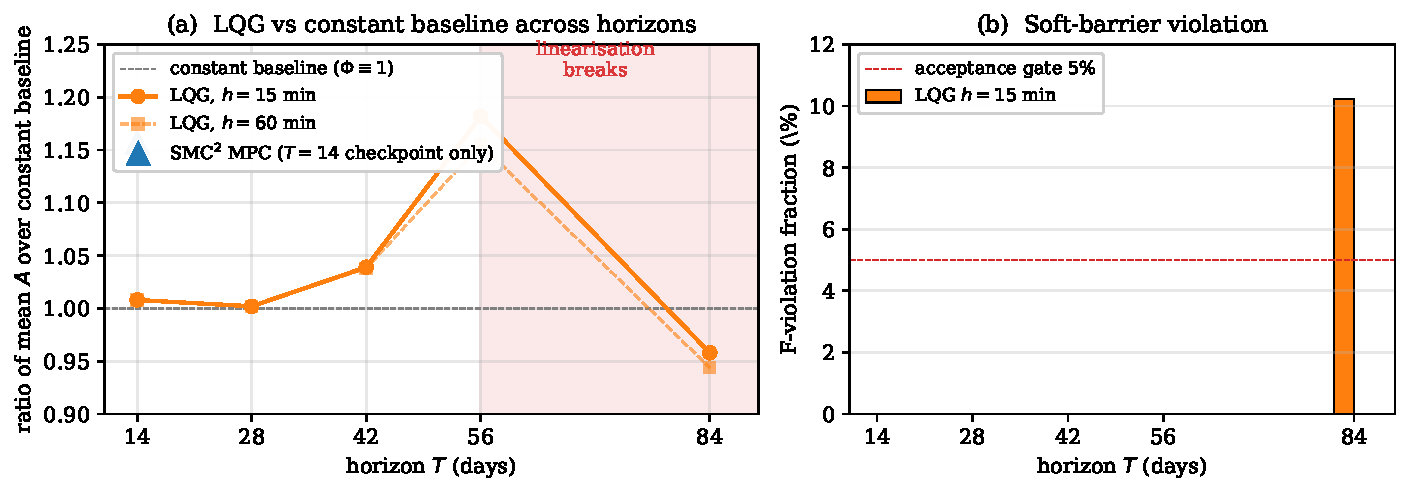
\includegraphics[width=\linewidth]{figures/fig_lqg_horizon.pdf}
\caption{(a) LQG ratio against the constant-$\Phi=1$ baseline as a
function of horizon. The dashed line at $1.0$ is the baseline; the
LQG curve rises through intermediate horizons, peaks near $T = 56$ d,
and crashes back through $1.0$ at $T = 84$ d. (b) F-violation
fraction across horizons. The dashed line is the $5\%$ acceptance
gate of Section~\ref{sec:mpc-feasibility}; LQG honours it for
$T \le 56$ d, then shoots past at $T = 84$ d.}
\label{fig:lqg-horizon}
\end{figure}

The LQG schedule shape is gradually rising: mean $\Phi$ climbs from
$\approx 0.91$ at $T = 14$ d through to $\approx 1.41$ at $T = 56$ d,
respecting the symmetric quadratic $F$-penalty by staying moderate.
At $T = 84$ d the slowly unstable eigenvalue (S2) of
\eqref{eq:lqg-numbers} has had enough horizon to dominate the
Riccati cost-to-go, the gain pushes $\Phi$ to its upper bound, and
the symmetric penalty cannot enforce the asymmetric soft-plus
$F$-barrier of the true cost \eqref{eq:cost}.

\subsection{Head-to-head against SMC$^2$ MPC at \texorpdfstring{$T = 14$}{T=14}}\label{app:lqg-headtohead}

At $T = 14$ d -- the only horizon for which both the SMC${}^2$ MPC
and the LQG runs have committed checkpoints -- the head-to-head
comparison is unambiguous.

\begin{figure}[h]
\centering
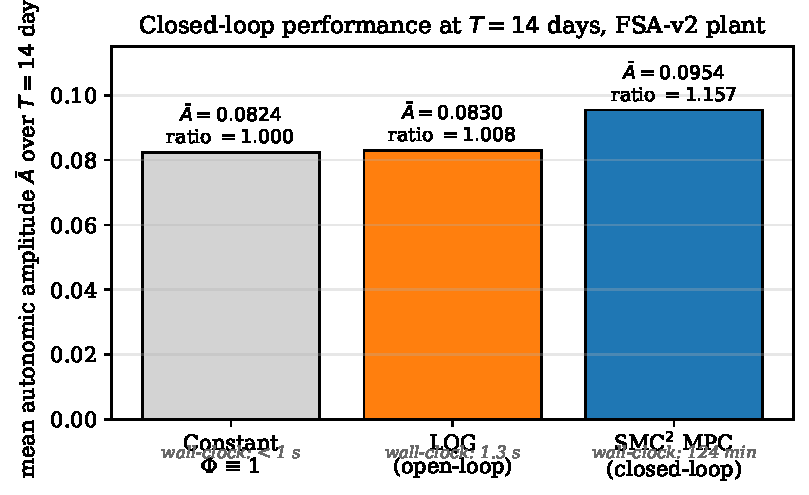
\includegraphics[width=0.65\linewidth]{figures/fig_t14_comparison.pdf}
\caption{Closed-loop performance at $T = 14$ d. The LQG schedule
delivers essentially the same mean amplitude as the constant
baseline (ratio $1.008$); the full SMC${}^2$ MPC delivers $+15.7\%$
over the same baseline (ratio $1.157$). Wall-clock cost is roughly
$5$--$6$ orders of magnitude apart.}
\label{fig:t14}
\end{figure}

The SMC${}^2$ MPC beats the tuned LQG by $\bar A_{\mathrm{MPC}}
- \bar A_{\mathrm{LQG}} = 0.0124$ in absolute terms, equivalently
$15$ percentage points of the constant-baseline reward, at a
wall-clock cost of $124$ minutes versus $1.3$ seconds. The non-linear
machinery is paying for the asymmetric $F$-barrier that LQG cannot
encode, and for a controller that sees the true cubic Stuart--Landau
dynamics through its plant simulator inside the cost Monte Carlo --
neither of which is available to a Riccati-based scheme. This is the
empirical answer to ``does the SMC${}^2$ machinery's compute cost
buy anything useful over a closed-form linear baseline?''. On
FSA-v2, with the cubic Stuart--Landau term that motivated the model
in the first place, it does.
